\begin{frame}{Power Analysis Attacks}

\begin{itemize}

	\item Power consumption during the execution of programs depends on intermediate values.

	\visible<2->{\item Power analysis attacks leverage this fact to find the secret key.}

\end{itemize}
\vspace{-4pt}

\only<3->{
\begin{figure}
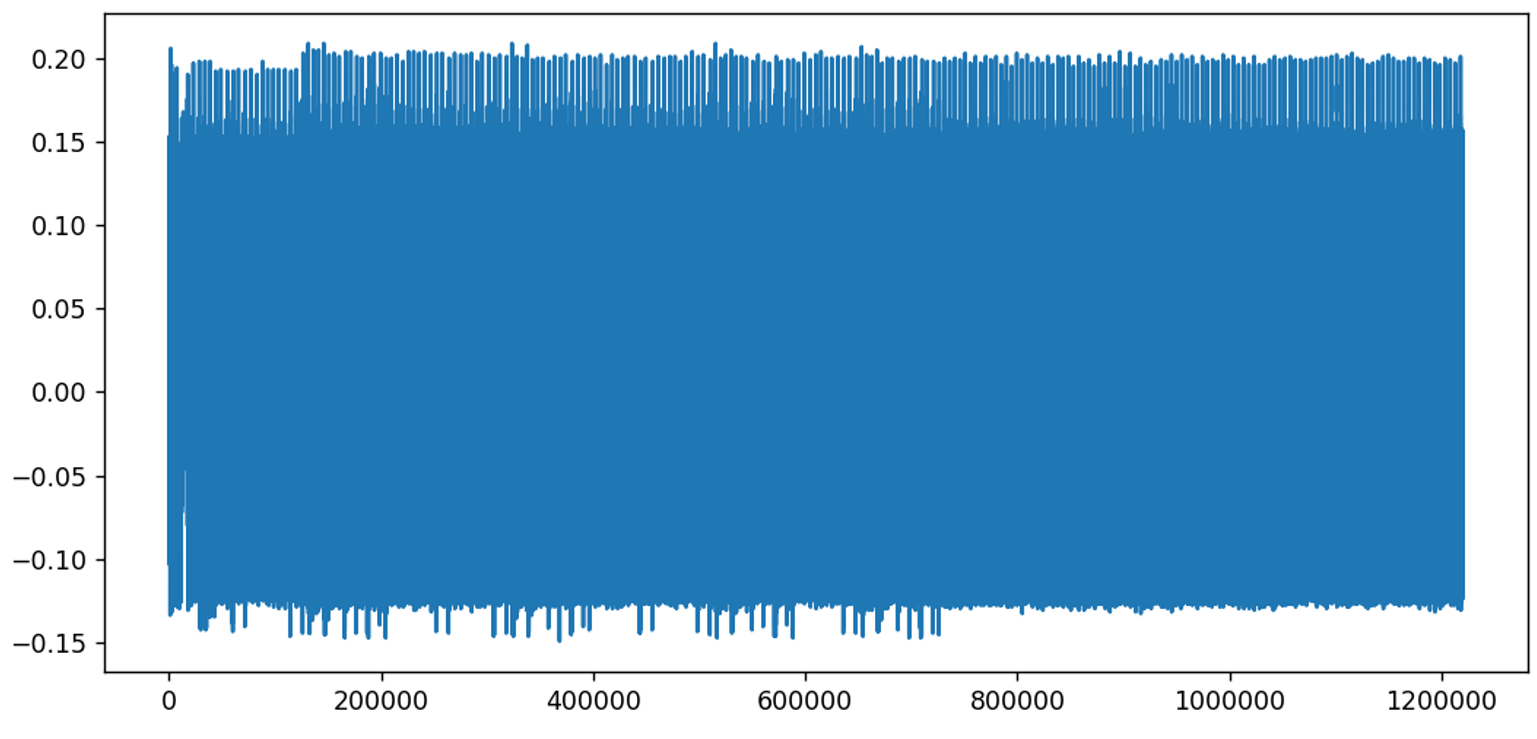
\includegraphics[width=.7\textwidth]{Figure/trace_example_ECC.png}
\vspace{-5pt}
\caption{An Example of a Power Trace}
\end{figure}
}

\end{frame}



\begin{frame}{Masking}

Masking defends against such threats by secret-sharing the sensitive variables.
\pause
\begin{itemize}
	\item Boolean Masking: A variable $x$ is split into $n$ shares $(x_i)_{1 \leq i \leq n}$ such that
	\[
	x = \bigoplus_{i=1}^n x_i
	\]
	\pause
	\item Arithmetic Masking: A variable $x$ is split into $n$ shares $(x_i)_{1 \leq i \leq n}$ (when stored in a $k$-bit register) such that
	\[
	x = \sum_{i=1}^n x_i \quad (\bmod\; 2^k)
	\]
\end{itemize}

\end{frame}


\begin{frame}{Masking}

\begin{itemize}
\item In each run, all $x_i$'s are randomized so that any $n-1$ shares of them are independently and uniformly distributed.
\pause
\item All operations need to be operated via shares.
\end{itemize}
\pause
For example, if $x$ is a secret variable, the operation $y \gets {\sf pt} \oplus x$ will become 
\[
	\begin{cases} y_1 \gets {\sf pt} \oplus x_1 \\ y_2 \gets x_2  \end{cases} \text{where } x_1,x_2 \text{ are sampled uniformly such that } x_1 \oplus x_2 = x
\]

The variables with secret information are splitted into shares.

\end{frame}
